\documentclass[tikz,border=3pt]{standalone}
\usepackage{amsmath}
\usepackage{sansmath}
\usetikzlibrary{arrows.meta,calc,decorations.pathmorphing,positioning}

\definecolor{ink}{HTML}{263238}
\definecolor{muted}{HTML}{66747B}
\definecolor{film}{HTML}{F4E7B8}
\definecolor{sulfur}{HTML}{D8A91B}
\definecolor{accent}{HTML}{347D8C}
\definecolor{warm}{HTML}{C35B43}
\definecolor{softblue}{HTML}{DCEEF1}

\tikzset{
  font=\sffamily,
  >={Stealth[length=2.2mm,width=1.5mm]},
  axis/.style={draw=ink, line width=.65pt, -{Stealth}},
  fine/.style={draw=ink, line width=.65pt},
  note/.style={font=\sffamily\scriptsize, text=muted, align=center},
  event/.style={circle, draw=accent, fill=white, line width=.75pt,
                minimum size=2.4mm, inner sep=0pt},
  trap/.style={draw=warm, line width=.65pt}
}

\begin{document}
\sansmath
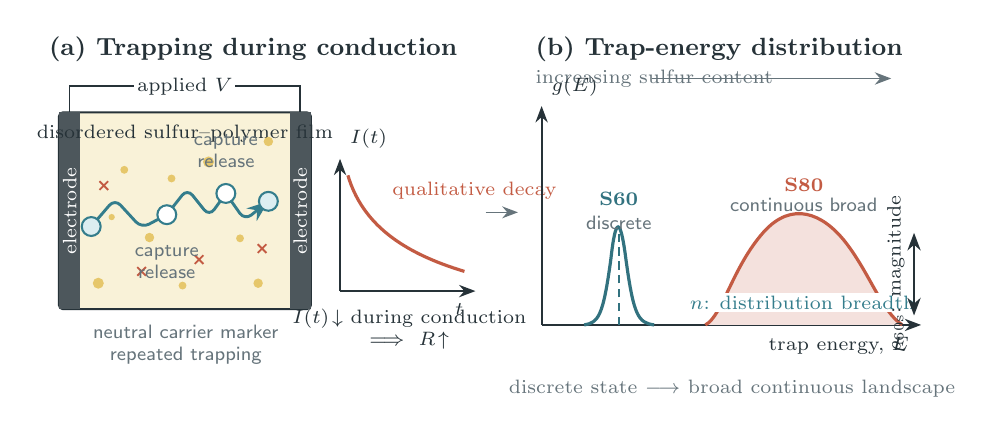
\begin{tikzpicture}[x=1cm,y=1cm]

% Panel A: biased cell, repeated capture/release, and qualitative decay.
\node[font=\bfseries\small, anchor=west, text=ink] at (0,4.55) {(a) Trapping during conduction};

\draw[rounded corners=1.5pt, fill=film!55, draw=ink, line width=.75pt]
  (0.25,1.25) rectangle (3.45,3.75);
\fill[ink!82] (0.25,1.25) rectangle (0.52,3.75);
\fill[ink!82] (3.18,1.25) rectangle (3.45,3.75);
\node[rotate=90, font=\scriptsize, text=white] at (0.385,2.50) {electrode};
\node[rotate=90, font=\scriptsize, text=white] at (3.315,2.50) {electrode};
\node[font=\scriptsize, text=ink] at (1.85,3.48) {disordered sulfur--polymer film};

% Sparse disorder texture and unassigned trap-site marks.
\foreach \x/\y/\r in {0.75/1.58/0.07,1.08/3.02/0.05,1.40/2.16/0.06,
  1.82/1.55/0.05,2.15/3.12/0.07,2.55/2.15/0.05,2.91/3.38/0.06,
  0.92/2.42/0.04,1.68/2.91/0.05,2.78/1.58/0.06}
  \fill[sulfur!65] (\x,\y) circle (\r);
\foreach \x/\y in {0.82/2.82,1.30/1.73,1.62/2.45,2.03/1.88,2.37/2.72,2.83/2.02}
  \draw[trap] (\x-0.055,\y-0.055)--(\x+0.055,\y+0.055)
              (\x-0.055,\y+0.055)--(\x+0.055,\y-0.055);

% Applied voltage is shown without assigning carrier polarity.
\draw[fine] (0.385,3.75) -- (0.385,4.08) -- (3.315,4.08) -- (3.315,3.75);
\node[fill=white, inner sep=1pt, font=\scriptsize, text=ink] at (1.85,4.08)
  {applied $V$};

% A tortuous trajectory with distinct capture and release moments.
\draw[accent, line width=1.05pt, rounded corners=3pt, -{Stealth}]
  (0.66,2.30) -- (0.96,2.65) -- (1.30,2.28) -- (1.62,2.45)
  -- (1.88,2.78) -- (2.16,2.43) -- (2.37,2.72)
  -- (2.61,2.38) -- (2.91,2.62);
\node[event, fill=softblue] at (0.66,2.30) {};
\node[event] at (1.62,2.45) {};
\node[event] at (2.37,2.72) {};
\node[event, fill=softblue] at (2.91,2.62) {};
\node[note, anchor=north] at (1.62,2.18) {capture\\release};
\node[note, anchor=south] at (2.37,2.92) {capture\\release};
\node[note, anchor=north west] at (0.56,1.17) {neutral carrier marker\\repeated trapping};

% Qualitative transient-current inset: intentionally no ticks or data points.
\begin{scope}[shift={(3.82,1.48)}]
  \draw[axis] (0,0) -- (1.72,0) node[below left=1pt, font=\scriptsize, text=ink] {$t$};
  \draw[axis] (0,0) -- (0,1.68) node[above right=0pt, font=\scriptsize, text=ink] {$I(t)$};
  \draw[warm, line width=1.15pt]
    (0.10,1.47) .. controls (0.28,.86) and (0.78,.49) .. (1.58,.25);
  \node[font=\scriptsize, text=warm, anchor=west] at (.54,1.28)
    {qualitative decay};
  \node[font=\scriptsize, text=ink, align=center] at (.88,-.48)
    {$I(t)\!\downarrow$ during conduction\\$\Longrightarrow\ R\!\uparrow$};
\end{scope}

\draw[muted, line width=.6pt, -{Stealth}] (5.67,2.48) -- (6.08,2.48);

% Panel B: independent distribution breadth and magnitude cues.
\node[font=\bfseries\small, anchor=west, text=ink] at (6.18,4.55)
  {(b) Trap-energy distribution};
\node[font=\scriptsize, anchor=west, text=muted] at (6.18,4.18)
  {increasing sulfur content};
\draw[muted, line width=.65pt, -{Stealth}] (7.78,4.18) -- (10.82,4.18);

\begin{scope}[shift={(6.38,1.05)}]
  \draw[axis] (0,0) -- (4.82,0) node[below left=1pt, font=\scriptsize, text=ink]
    {trap energy, $E$};
  \draw[axis] (0,0) -- (0,2.78) node[above right=0pt, font=\scriptsize, text=ink]
    {$g(E)$};

  % S60: one discrete, narrow state.
  \draw[accent!85!ink, line width=1.15pt]
    (.54,0) .. controls (.72,.03) and (.78,.10) .. (.88,.84)
    .. controls (.94,1.38) and (1.00,1.38) .. (1.07,.84)
    .. controls (1.17,.10) and (1.23,.03) .. (1.43,0);
  \draw[accent!85!ink, densely dashed, line width=.55pt] (.98,0)--(.98,1.25);
  \node[font=\bfseries\scriptsize, text=accent!85!ink] at (.98,1.60) {S60};
  \node[note] at (.98,1.30) {discrete};

  % S80: broad continuous distribution, separated spatially for legibility.
  \path[fill=warm!18, draw=none]
    (2.08,0) .. controls (2.30,.12) and (2.42,.73) .. (2.82,1.18)
    .. controls (3.18,1.58) and (3.57,1.42) .. (3.86,1.05)
    .. controls (4.17,.65) and (4.32,.17) .. (4.58,0) -- cycle;
  \draw[warm, line width=1.15pt]
    (2.08,0) .. controls (2.30,.12) and (2.42,.73) .. (2.82,1.18)
    .. controls (3.18,1.58) and (3.57,1.42) .. (3.86,1.05)
    .. controls (4.17,.65) and (4.32,.17) .. (4.58,0);
  \node[font=\bfseries\scriptsize, text=warm] at (3.33,1.78) {S80};
  \node[note] at (3.33,1.52) {continuous broad};

  % Horizontal n span: breadth only.
  \draw[accent, line width=.75pt, {Stealth}-{Stealth}] (2.23,.28)--(4.40,.28);
  \node[fill=white, inner sep=1pt, font=\scriptsize, text=accent] at (3.315,.28)
    {$n$: distribution breadth};

  % Independent vertical magnitude cue, deliberately outside the distributions.
  \draw[ink, line width=.75pt, {Stealth}-{Stealth}] (4.73,.12)--(4.73,1.17);
  \node[font=\scriptsize, text=ink, rotate=90, anchor=south] at (4.73,.645)
    {$\rho_{60\mathrm{s}}$: magnitude};
\end{scope}

\node[font=\scriptsize, text=muted, align=center] at (8.80,.24)
  {discrete state $\longrightarrow$ broad continuous landscape};

\end{tikzpicture}
\end{document}
